\chapter{Lösungsansatz zur Klassifikation}
In diesem Kapitel geht es um die Strategie, wie eine Klassifikation der
Hunderassen für den großen (120 Klassen) und den kleinen (5 Klassen) Datensatz
mittels mehrerer Neuronaler Netze erreicht werden kann.

\section{Größe der Bilder}
Höhe und Breite der Bilder sind unterschiedlich im großen Datensatz, wie in
\autoref{fig:scatter_groß} dargestellt.

\begin{figure}
  \centering
  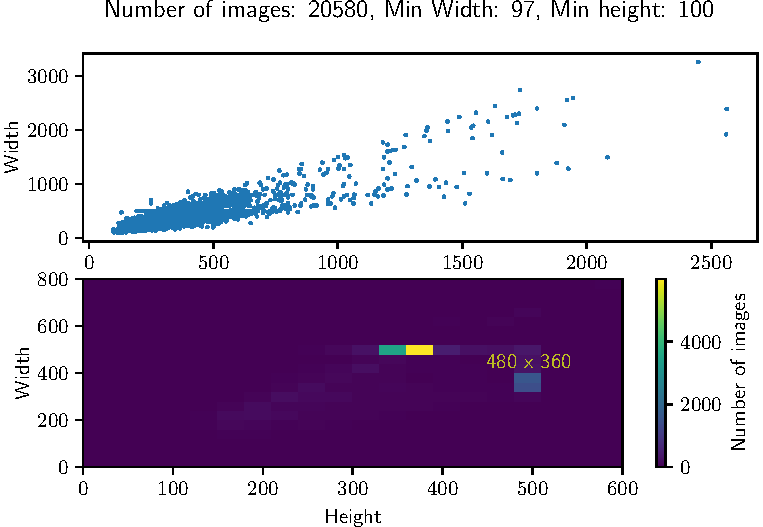
\includegraphics[scale=0.8]{pics/width_height_scatter_hist2d.pdf}
  \caption{Oben: Scatter-Plot der Höhen- und Breitenverteilung der Bilder aus dem großen Datensatz.
  Unten: Zweidimensionales Histogramm der Höhen- und Breitenverteilung.
  Die gelbe Größe entspricht der am häufigsten auftretenden Kombination
  aus Breite und Höhe.}
  \label{fig:scatter_groß}
\end{figure}

Die minimale Breite liegt bei 97 Pixeln und die minimale Höhe bei 100 Pixeln.
Prinzipiell arbeiten die verwendeten Neuronalen Netze ohne definierte Input
size, allerdings müssen die Bilder auf eine Größe gebracht werden, da
\texttt{numpy arrays} eine definierte Größe haben müssen. Eine Möglichkeit wäre
es nun, alle Bilder auf diese minimale Größe zu resizen. Damit würde allerdings
ein Informationsverlust einhergehen. Aus diesem Grund wurde ein zu Teilen
selbstgeschriebener \texttt{Datagenerator} verwendet, der die Bilder batchwise
lädt und batchwise auf das Minimum im Batch resized. Auf diese Weise ist der
Informationsverlust geringer als alle Bilder auf 97x100 zu resizen.

In \autoref{fig:scatter_klein} ist die Höhen- und Breitenverteilung auch für
den kleinen Datensatz dargestellt.

\begin{figure}
  \centering
  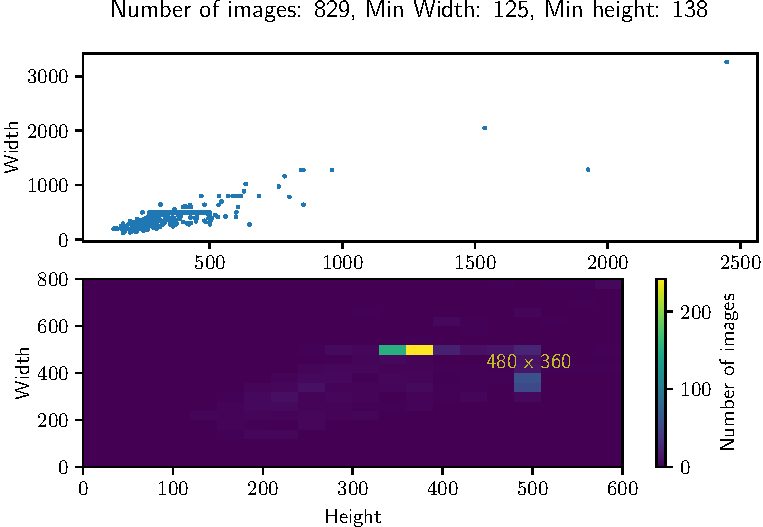
\includegraphics[scale=0.8]{pics/width_height_scatter_hist2d_klein.pdf}
  \caption{Oben: Scatter-Plot der Höhen- und Breitenverteilung der Bilder aus
  dem kleinen Datensatz.
  Unten: Zweidimensionales Histogramm der Höhen- und Breitenverteilung.
  Die gelbe Größe entspricht der am häufigsten auftretenden Kombination
  aus Breite und Höhe.}
  \label{fig:scatter_klein}
\end{figure}

Auch für den kleinen Datensatz wird der oben erwähnte \texttt{Datagenerator}
verwendet. Somit wird auch hier batchwise auf das Minimum resized.

\section{Data Augmentation}
Wie bereits in \autoref{chap:datensatz} dargestellt, entfallen auf jede Klasse nur ungefähr
150 Bilder, was eine sehr geringe Statistik darstellt. Aus diesem Grund wurde
Data Augmentation verwendet. Das bedeutet, dass bei jedem neuen Aufruf des \texttt{Datagenerators}
nach dem Resizen das Bild um einen zufälligen Winkel zwischen \SI{-30}{\degree}
und \SI{30}{\degree} rotiert wird. Dabei aufstehende Leerflächen werden geschwärzt.
Dann wird mit \SI{50}{\percent} Wahrscheinlichkeit das Bild in x- und y-Richtung verschoben
oder ein Zoom in x- und y-Richtung durchgeführt. Damit bei diesen Transformationen
der Hund noch immer komplett zu sehen ist und nicht z.\,B. durch die Verschiebung
nur noch ein Teil des Hundes zu sehen ist, wird vorher aufgrund der Bounding Boxes,
die im Datensatz gegeben sind, das Zoom- bzw. Translationslimit bestimmt.
